\subsection{Dataset Description}
The initial state-labeled exploratory dataset contained 37,028 aggregate records over 60 geographic categories. Average observed payment had a mean of \$327.78, median of \$39.56, and standard deviation of \$1,181.06, demonstrating a wide distribution of record-level payment values (Table~\ref{tab:description}). The primary 51-area dataset retained 36,528 rows, with mean and median observed payments of \$330.37 and \$39.76, respectively.
\begin{table}[!htbp]\centering
\caption{Dataset composition and observed-payment summary.}\label{tab:description}
\begin{tabular}{lrr}\toprule
Measure & Exploratory & Primary \\\midrule
Records & 37,028 & 36,528\\
Geographic categories & 60 & 51\\
HCPCS codes & 1,250 & 1,250\\
Mean payment (USD) & 327.78 & 330.37\\
Median payment (USD) & 39.56 & 39.76\\
\bottomrule\end{tabular}\end{table}
\begin{figure}[!htbp]\centering
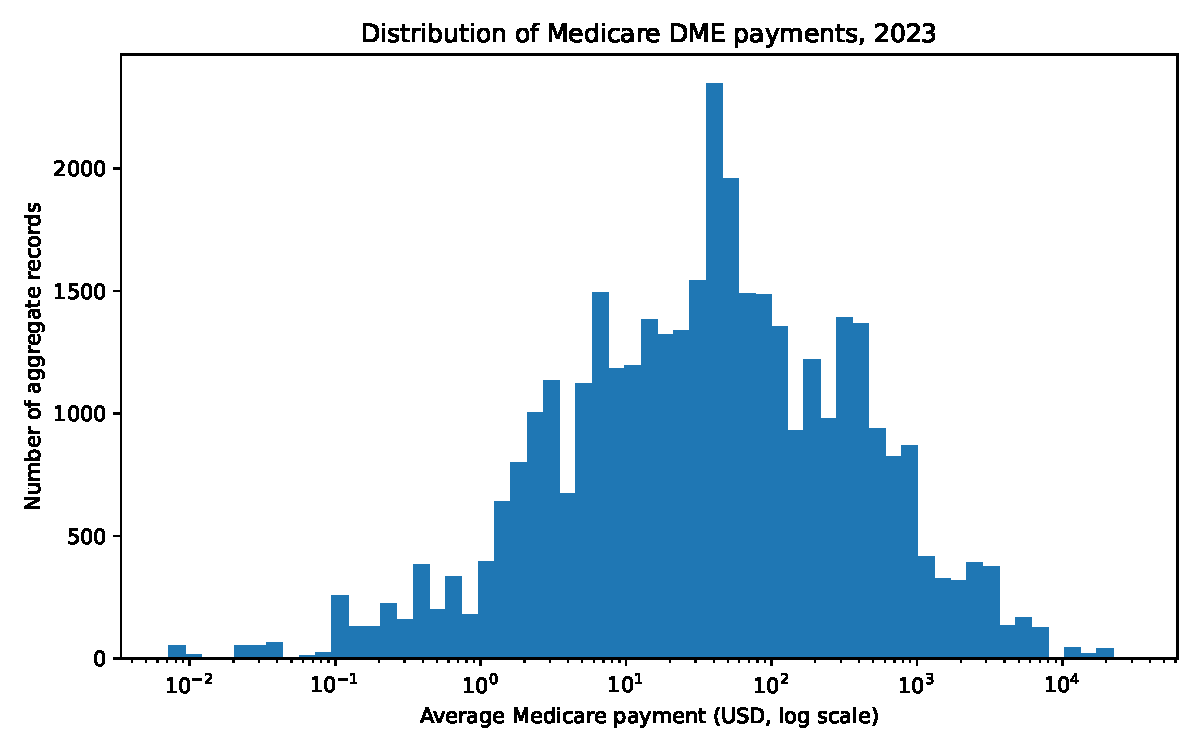
\includegraphics[width=.61\linewidth]{payment_distribution.pdf}
\caption{Observed average Medicare DME payments in the preliminary 60-category exploratory dataset, displayed on a logarithmic horizontal axis.}\label{fig:distribution}\end{figure}
\begin{figure}[!htbp]\centering
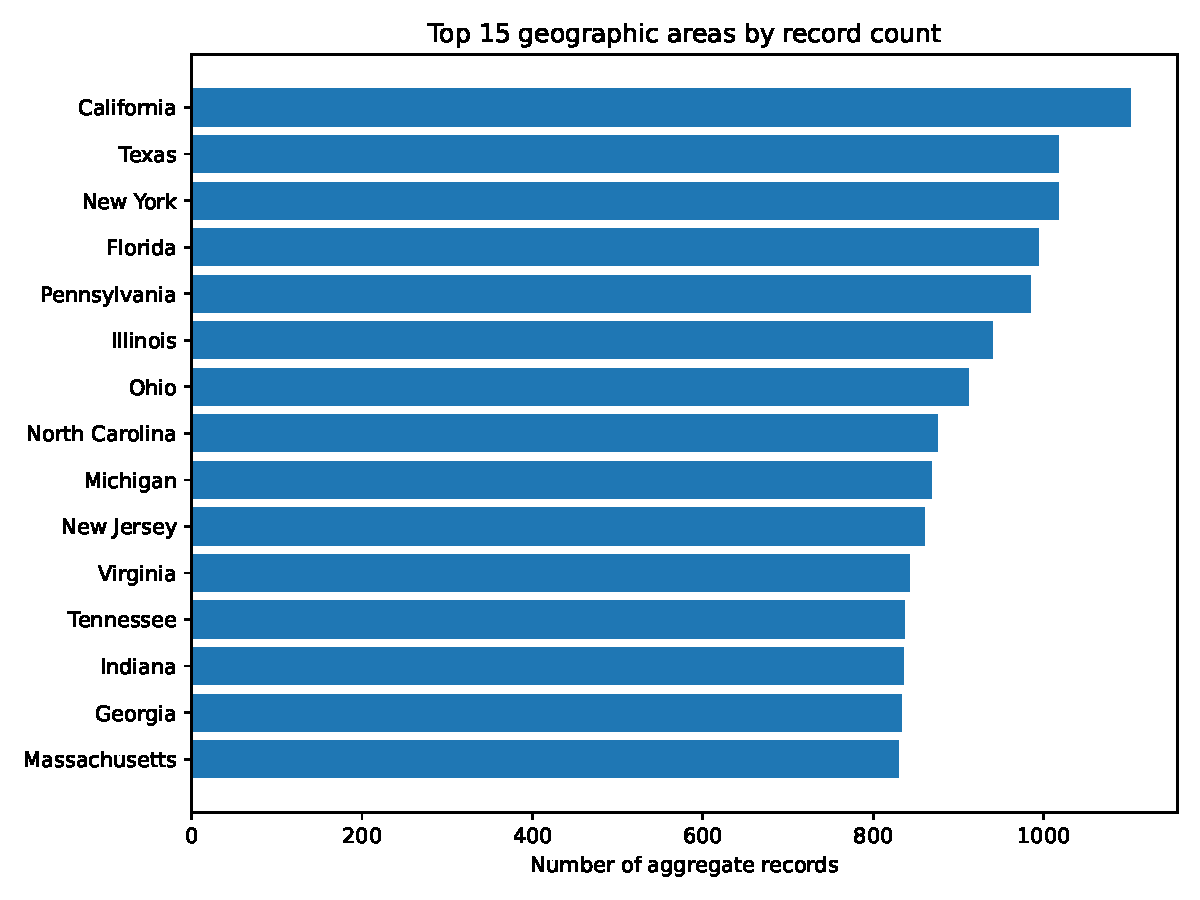
\includegraphics[width=.61\linewidth]{geographic_coverage.pdf}
\caption{Fifteen geographic categories with the greatest number of aggregate records in the exploratory dataset.}\label{fig:coverage}\end{figure}

\subsection{Preliminary Baselines and Geographic Holdout}
On the initial random 80/20 split of the 60-category dataset, the global-mean baseline had an MAE of \$458.62 and an RMSE of \$1,210.88. The HCPCS-mean baseline reduced these to \$48.97 and \$265.43. Across 30 preliminary split seeds, mean random-split HCPCS MAE was \$49.07 and mean geographic-holdout MAE was \$47.60. Geographic holdout produced larger MAE in 12 of 30 comparisons, so these experiments do not support a claim that random splitting invariably understates error.
\begin{table}[!htbp]\centering
\caption{Preliminary results on the 60-category population.}\label{tab:preliminary}
\begin{tabular}{lrr}\toprule
Random-split model & MAE (USD) & RMSE (USD)\\\midrule
Global training mean & 458.62 & 1210.88\\
HCPCS training mean & 48.97 & 265.43\\
\bottomrule\end{tabular}\end{table}
\subsection{Geographic Reliability and HCPCS Coverage}
For 51-area leave-one-area-out evaluation, the HCPCS-only baseline achieved an actual-payment micro MAE of \$47.84 and macro area MAE of \$46.27. Texas had the largest observed area MAE, \$103.55. The 36,391 test records with codes observed in training had MAE \$45.21. Only 137 records (0.38\%) had unseen HCPCS codes, but these had MAE \$747.00 and contributed 5.86\% of total absolute prediction error (Table~\ref{tab:coverage}).
\begin{table}[!htbp]\centering
\caption{Known versus unseen HCPCS code errors, 51-area HCPCS-only baseline.}\label{tab:coverage}
\begin{tabular}{lrrr}\toprule
Code status & Records & MAE (USD) & Error share\\\midrule
Known & 36,391 & 45.21 & 94.14\%\\
Unseen & 137 & 747.00 & 5.86\%\\
\bottomrule\end{tabular}\end{table}

\subsection{Payment Standardization and Within-Group Variation}
Among the 916 HCPCS/rental groups present in at least ten areas, the mean observed-payment CV was 0.09059 and the corresponding mean standardized-payment CV was 0.04744. Standardized CV was smaller in 805 groups (87.9\%), larger in 95 groups, and equal in 16 groups (Table~\ref{tab:cv}). The distribution of paired coefficients is displayed in Figure~\ref{fig:cv}. Since standardization is designed partly to remove policy-based payment differences, this result is interpreted as a descriptive check rather than as a novel standardization method.
\begin{table}[!htbp]\centering
\caption{Actual versus standardized within-group geographic variation.}\label{tab:cv}
\begin{tabular}{lr}\toprule
Measure & Value\\\midrule
Eligible HCPCS/rental groups & 916\\
Mean observed-payment CV & 0.09059\\
Mean standardized-payment CV & 0.04744\\
Groups with lower standardized CV & 805\\
Groups with higher standardized CV & 95\\
Groups with equal CV & 16\\
\bottomrule\end{tabular}\end{table}
\begin{figure}[!htbp]\centering
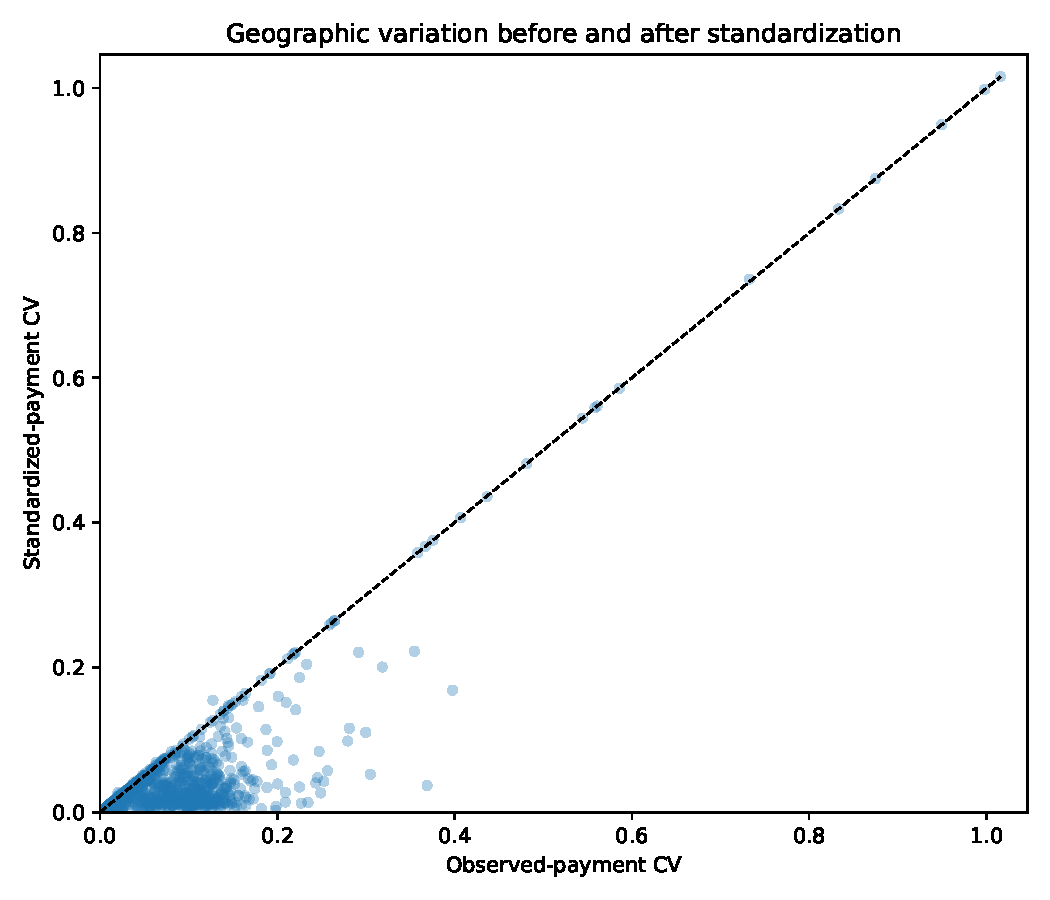
\includegraphics[width=.61\linewidth]{standardization_cv_comparison.pdf}
\caption{Observed and standardized coefficients of variation across 916 comparable HCPCS/rental groups. The dashed diagonal represents equal variation.}\label{fig:cv}\end{figure}

\subsection{Paired Target Prediction and Rental-Aware Analysis}
In paired leave-one-area-out testing, the HCPCS-only baseline had an actual-payment micro MAE of \$47.84, compared with \$38.88 for the standardized-payment target. The analogous RMSEs were \$290.78 and \$284.49. Both MAE and normalized MAE were smaller for the standardized target in every one of the 51 held-out geographic areas.

Including rental classification in the group-mean baseline reduced actual-payment MAE to \$19.89 and standardized-payment MAE to \$10.30, corresponding to reductions of 58.4\% and 73.5\% relative to the HCPCS-only baselines for the respective targets. Under the rental-aware specification, standardized-target MAE was lower in all 51 areas, while the worst-area MAEs were \$66.42 and \$54.63 for actual and standardized payments, respectively (Table~\ref{tab:models}). The improvements in RMSE were substantially smaller than those in MAE, indicating that large residual errors remain influential.
\begin{table}[!htbp]\centering\small
\caption{Leave-one-area-out prediction errors on the 51-area primary population. Each target is predicted separately.}\label{tab:models}
\begin{tabular}{llrrrr}\toprule
Model & Target & MAE & RMSE & NMAE\% & Worst MAE\\\midrule
HCPCS & Actual & 47.84 & 290.78 & 14.48 & 103.55\\
HCPCS & Standardized & 38.88 & 284.49 & 11.71 & 92.72\\
HCPCS+rental & Actual & 19.89 & 185.67 & 6.02 & 66.42\\
HCPCS+rental & Standardized & 10.30 & 182.01 & 3.10 & 54.63\\
\bottomrule\end{tabular}\end{table}
